\documentclass[twoside]{book}

% Packages required by doxygen
\usepackage{fixltx2e}
\usepackage{calc}
\usepackage{doxygen}
\usepackage[export]{adjustbox} % also loads graphicx
\usepackage{graphicx}
\usepackage[utf8]{inputenc}
\usepackage{makeidx}
\usepackage{multicol}
\usepackage{multirow}
\PassOptionsToPackage{warn}{textcomp}
\usepackage{textcomp}
\usepackage[nointegrals]{wasysym}
\usepackage[table]{xcolor}

% Font selection
\usepackage[T1]{fontenc}
\usepackage[scaled=.90]{helvet}
\usepackage{courier}
\usepackage{amssymb}
\usepackage{sectsty}
\renewcommand{\familydefault}{\sfdefault}
\allsectionsfont{%
  \fontseries{bc}\selectfont%
  \color{darkgray}%
}
\renewcommand{\DoxyLabelFont}{%
  \fontseries{bc}\selectfont%
  \color{darkgray}%
}
\newcommand{\+}{\discretionary{\mbox{\scriptsize$\hookleftarrow$}}{}{}}

% Page & text layout
\usepackage{geometry}
\geometry{%
  a4paper,%
  top=2.5cm,%
  bottom=2.5cm,%
  left=2.5cm,%
  right=2.5cm%
}
\tolerance=750
\hfuzz=15pt
\hbadness=750
\setlength{\emergencystretch}{15pt}
\setlength{\parindent}{0cm}
\setlength{\parskip}{3ex plus 2ex minus 2ex}
\makeatletter
\renewcommand{\paragraph}{%
  \@startsection{paragraph}{4}{0ex}{-1.0ex}{1.0ex}{%
    \normalfont\normalsize\bfseries\SS@parafont%
  }%
}
\renewcommand{\subparagraph}{%
  \@startsection{subparagraph}{5}{0ex}{-1.0ex}{1.0ex}{%
    \normalfont\normalsize\bfseries\SS@subparafont%
  }%
}
\makeatother

% Headers & footers
\usepackage{fancyhdr}
\pagestyle{fancyplain}
\fancyhead[LE]{\fancyplain{}{\bfseries\thepage}}
\fancyhead[CE]{\fancyplain{}{}}
\fancyhead[RE]{\fancyplain{}{\bfseries\leftmark}}
\fancyhead[LO]{\fancyplain{}{\bfseries\rightmark}}
\fancyhead[CO]{\fancyplain{}{}}
\fancyhead[RO]{\fancyplain{}{\bfseries\thepage}}
\fancyfoot[LE]{\fancyplain{}{}}
\fancyfoot[CE]{\fancyplain{}{}}
\fancyfoot[RE]{\fancyplain{}{\bfseries\scriptsize Generated by Doxygen }}
\fancyfoot[LO]{\fancyplain{}{\bfseries\scriptsize Generated by Doxygen }}
\fancyfoot[CO]{\fancyplain{}{}}
\fancyfoot[RO]{\fancyplain{}{}}
\renewcommand{\footrulewidth}{0.4pt}
\renewcommand{\chaptermark}[1]{%
  \markboth{#1}{}%
}
\renewcommand{\sectionmark}[1]{%
  \markright{\thesection\ #1}%
}

% Indices & bibliography
\usepackage{natbib}
\usepackage[titles]{tocloft}
\setcounter{tocdepth}{3}
\setcounter{secnumdepth}{5}
\makeindex

% Hyperlinks (required, but should be loaded last)
\usepackage{ifpdf}
\ifpdf
  \usepackage[pdftex,pagebackref=true]{hyperref}
\else
  \usepackage[ps2pdf,pagebackref=true]{hyperref}
\fi
\hypersetup{%
  colorlinks=true,%
  linkcolor=blue,%
  citecolor=blue,%
  unicode%
}

% Custom commands
\newcommand{\clearemptydoublepage}{%
  \newpage{\pagestyle{empty}\cleardoublepage}%
}

\usepackage{caption}
\captionsetup{labelsep=space,justification=centering,font={bf},singlelinecheck=off,skip=4pt,position=top}

%===== C O N T E N T S =====

\begin{document}

% Titlepage & ToC
\hypersetup{pageanchor=false,
             bookmarksnumbered=true,
             pdfencoding=unicode
            }
\pagenumbering{roman}
\begin{titlepage}
\vspace*{7cm}
\begin{center}%
{\Large Simple Instant Messaging Application }\\
\vspace*{1cm}
{\large Generated by Doxygen 1.8.11}\\
\end{center}
\end{titlepage}
\clearemptydoublepage
\tableofcontents
\clearemptydoublepage
\pagenumbering{arabic}
\hypersetup{pageanchor=true}

%--- Begin generated contents ---
\chapter{Hierarchical Index}
\section{Class Hierarchy}
This inheritance list is sorted roughly, but not completely, alphabetically\+:\begin{DoxyCompactList}
\item \contentsline{section}{Conn}{\pageref{classConn}}{}
\item \contentsline{section}{Context}{\pageref{classContext}}{}
\item \contentsline{section}{Message}{\pageref{structMessage}}{}
\item runtime\+\_\+error\begin{DoxyCompactList}
\item \contentsline{section}{Cmd\+Failed}{\pageref{classCmdFailed}}{}
\item \contentsline{section}{Invalid\+Message}{\pageref{classInvalidMessage}}{}
\item \contentsline{section}{Network\+Error}{\pageref{classNetworkError}}{}
\end{DoxyCompactList}
\item \contentsline{section}{User}{\pageref{structUser}}{}
\end{DoxyCompactList}

\chapter{Class Index}
\section{Class List}
Here are the classes, structs, unions and interfaces with brief descriptions\+:\begin{DoxyCompactList}
\item\contentsline{section}{\hyperlink{classCmdFailed}{Cmd\+Failed} }{\pageref{classCmdFailed}}{}
\item\contentsline{section}{\hyperlink{classConn}{Conn} \\*Connection manager }{\pageref{classConn}}{}
\item\contentsline{section}{\hyperlink{classContext}{Context} \\*\hyperlink{classContext}{Context} of a connection }{\pageref{classContext}}{}
\item\contentsline{section}{\hyperlink{classInvalidMessage}{Invalid\+Message} }{\pageref{classInvalidMessage}}{}
\item\contentsline{section}{\hyperlink{structMessage}{Message} }{\pageref{structMessage}}{}
\item\contentsline{section}{\hyperlink{classNetworkError}{Network\+Error} }{\pageref{classNetworkError}}{}
\item\contentsline{section}{\hyperlink{structUser}{User} }{\pageref{structUser}}{}
\end{DoxyCompactList}

\chapter{File Index}
\section{File List}
Here is a list of all files with brief descriptions\+:\begin{DoxyCompactList}
\item\contentsline{section}{\hyperlink{CmdFailed_8h}{Cmd\+Failed.\+h} }{\pageref{CmdFailed_8h}}{}
\item\contentsline{section}{\hyperlink{config_8h}{config.\+h} }{\pageref{config_8h}}{}
\item\contentsline{section}{\hyperlink{Conn_8cpp}{Conn.\+cpp} }{\pageref{Conn_8cpp}}{}
\item\contentsline{section}{\hyperlink{Conn_8h}{Conn.\+h} }{\pageref{Conn_8h}}{}
\item\contentsline{section}{\hyperlink{Context_8cpp}{Context.\+cpp} }{\pageref{Context_8cpp}}{}
\item\contentsline{section}{\hyperlink{Context_8h}{Context.\+h} }{\pageref{Context_8h}}{}
\item\contentsline{section}{\hyperlink{InvalidMessage_8h}{Invalid\+Message.\+h} }{\pageref{InvalidMessage_8h}}{}
\item\contentsline{section}{\hyperlink{main_8cpp}{main.\+cpp} }{\pageref{main_8cpp}}{}
\item\contentsline{section}{\hyperlink{Message_8h}{Message.\+h} }{\pageref{Message_8h}}{}
\item\contentsline{section}{\hyperlink{NetworkError_8h}{Network\+Error.\+h} }{\pageref{NetworkError_8h}}{}
\item\contentsline{section}{\hyperlink{User_8h}{User.\+h} }{\pageref{User_8h}}{}
\end{DoxyCompactList}

\chapter{Class Documentation}
\hypertarget{classCmdFailed}{}\section{Cmd\+Failed Class Reference}
\label{classCmdFailed}\index{Cmd\+Failed@{Cmd\+Failed}}


{\ttfamily \#include $<$Cmd\+Failed.\+h$>$}



Inheritance diagram for Cmd\+Failed\+:
\nopagebreak
\begin{figure}[H]
\begin{center}
\leavevmode
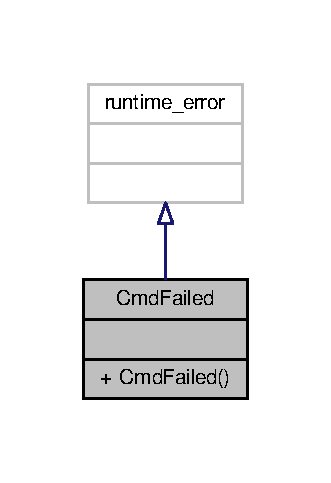
\includegraphics[width=159pt]{classCmdFailed__inherit__graph}
\end{center}
\end{figure}


Collaboration diagram for Cmd\+Failed\+:
\nopagebreak
\begin{figure}[H]
\begin{center}
\leavevmode
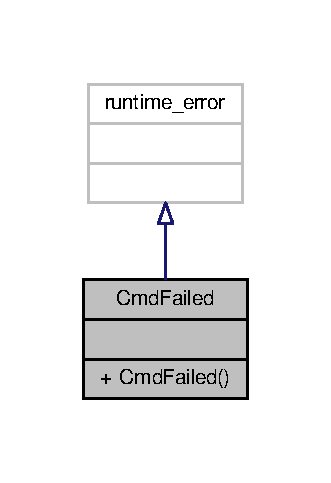
\includegraphics[width=159pt]{classCmdFailed__coll__graph}
\end{center}
\end{figure}
\subsection*{Public Member Functions}
\begin{DoxyCompactItemize}
\item 
\hyperlink{classCmdFailed_a63bc8a9d1e23555dde951446f6c33d62}{Cmd\+Failed} (const std\+::string \&what)
\end{DoxyCompactItemize}


\subsection{Constructor \& Destructor Documentation}
\index{Cmd\+Failed@{Cmd\+Failed}!Cmd\+Failed@{Cmd\+Failed}}
\index{Cmd\+Failed@{Cmd\+Failed}!Cmd\+Failed@{Cmd\+Failed}}
\subsubsection[{\texorpdfstring{Cmd\+Failed(const std\+::string \&what)}{CmdFailed(const std::string &what)}}]{\setlength{\rightskip}{0pt plus 5cm}Cmd\+Failed\+::\+Cmd\+Failed (
\begin{DoxyParamCaption}
\item[{const std\+::string \&}]{what}
\end{DoxyParamCaption}
)\hspace{0.3cm}{\ttfamily [inline]}}\hypertarget{classCmdFailed_a63bc8a9d1e23555dde951446f6c33d62}{}\label{classCmdFailed_a63bc8a9d1e23555dde951446f6c33d62}


The documentation for this class was generated from the following file\+:\begin{DoxyCompactItemize}
\item 
\hyperlink{CmdFailed_8h}{Cmd\+Failed.\+h}\end{DoxyCompactItemize}

\hypertarget{classConn}{}\section{Conn Class Reference}
\label{classConn}\index{Conn@{Conn}}


Connection manager.  




{\ttfamily \#include $<$Conn.\+h$>$}



Collaboration diagram for Conn\+:
\nopagebreak
\begin{figure}[H]
\begin{center}
\leavevmode
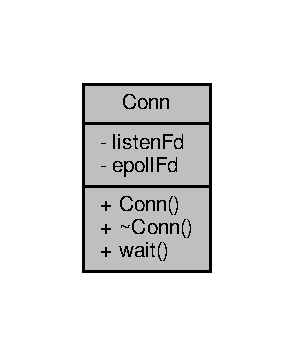
\includegraphics[width=141pt]{classConn__coll__graph}
\end{center}
\end{figure}
\subsection*{Public Member Functions}
\begin{DoxyCompactItemize}
\item 
\hyperlink{classConn_a7312553a7ce3efd712427ccd5a0106c6}{Conn} (unsigned short port)
\begin{DoxyCompactList}\small\item\em Setup listening on a T\+CP port. \end{DoxyCompactList}\item 
\hyperlink{classConn_a45fa096c27a1cdbeb295c903045ce071}{$\sim$\+Conn} ()
\begin{DoxyCompactList}\small\item\em Close the file descriptors. \end{DoxyCompactList}\item 
{\footnotesize template$<$class Callback $>$ }\\void \hyperlink{classConn_a1c06e5cf18d612c261b49198c99fa0d6}{wait} (const Callback \&callback)
\begin{DoxyCompactList}\small\item\em Wait until a connection is readable This will block the thread forever. \end{DoxyCompactList}\end{DoxyCompactItemize}
\subsection*{Private Attributes}
\begin{DoxyCompactItemize}
\item 
int \hyperlink{classConn_a6af8be63a2c2649023fab93fa45f166a}{listen\+Fd}
\item 
int \hyperlink{classConn_a74f55eff092314212ed765eebe2022d5}{epoll\+Fd}
\end{DoxyCompactItemize}


\subsection{Detailed Description}
Connection manager. 

\subsection{Constructor \& Destructor Documentation}
\index{Conn@{Conn}!Conn@{Conn}}
\index{Conn@{Conn}!Conn@{Conn}}
\subsubsection[{\texorpdfstring{Conn(unsigned short port)}{Conn(unsigned short port)}}]{\setlength{\rightskip}{0pt plus 5cm}Conn\+::\+Conn (
\begin{DoxyParamCaption}
\item[{unsigned short}]{port}
\end{DoxyParamCaption}
)}\hypertarget{classConn_a7312553a7ce3efd712427ccd5a0106c6}{}\label{classConn_a7312553a7ce3efd712427ccd5a0106c6}


Setup listening on a T\+CP port. 


\begin{DoxyExceptions}{Exceptions}
{\em \hyperlink{classNetworkError}{Network\+Error}} & \\
\hline
\end{DoxyExceptions}
\index{Conn@{Conn}!````~Conn@{$\sim$\+Conn}}
\index{````~Conn@{$\sim$\+Conn}!Conn@{Conn}}
\subsubsection[{\texorpdfstring{$\sim$\+Conn()}{~Conn()}}]{\setlength{\rightskip}{0pt plus 5cm}Conn\+::$\sim$\+Conn (
\begin{DoxyParamCaption}
{}
\end{DoxyParamCaption}
)}\hypertarget{classConn_a45fa096c27a1cdbeb295c903045ce071}{}\label{classConn_a45fa096c27a1cdbeb295c903045ce071}


Close the file descriptors. 



\subsection{Member Function Documentation}
\index{Conn@{Conn}!wait@{wait}}
\index{wait@{wait}!Conn@{Conn}}
\subsubsection[{\texorpdfstring{wait(const Callback \&callback)}{wait(const Callback &callback)}}]{\setlength{\rightskip}{0pt plus 5cm}template$<$class Callback $>$ void Conn\+::wait (
\begin{DoxyParamCaption}
\item[{const Callback \&}]{callback}
\end{DoxyParamCaption}
)\hspace{0.3cm}{\ttfamily [inline]}}\hypertarget{classConn_a1c06e5cf18d612c261b49198c99fa0d6}{}\label{classConn_a1c06e5cf18d612c261b49198c99fa0d6}


Wait until a connection is readable This will block the thread forever. 


\begin{DoxyParams}{Parameters}
{\em callback} & \+: function(\+Context \&context) \\
\hline
\end{DoxyParams}


\subsection{Member Data Documentation}
\index{Conn@{Conn}!epoll\+Fd@{epoll\+Fd}}
\index{epoll\+Fd@{epoll\+Fd}!Conn@{Conn}}
\subsubsection[{\texorpdfstring{epoll\+Fd}{epollFd}}]{\setlength{\rightskip}{0pt plus 5cm}int Conn\+::epoll\+Fd\hspace{0.3cm}{\ttfamily [private]}}\hypertarget{classConn_a74f55eff092314212ed765eebe2022d5}{}\label{classConn_a74f55eff092314212ed765eebe2022d5}
\index{Conn@{Conn}!listen\+Fd@{listen\+Fd}}
\index{listen\+Fd@{listen\+Fd}!Conn@{Conn}}
\subsubsection[{\texorpdfstring{listen\+Fd}{listenFd}}]{\setlength{\rightskip}{0pt plus 5cm}int Conn\+::listen\+Fd\hspace{0.3cm}{\ttfamily [private]}}\hypertarget{classConn_a6af8be63a2c2649023fab93fa45f166a}{}\label{classConn_a6af8be63a2c2649023fab93fa45f166a}


The documentation for this class was generated from the following files\+:\begin{DoxyCompactItemize}
\item 
\hyperlink{Conn_8h}{Conn.\+h}\item 
\hyperlink{Conn_8cpp}{Conn.\+cpp}\end{DoxyCompactItemize}

\hypertarget{classContext}{}\section{Context Class Reference}
\label{classContext}\index{Context@{Context}}


\hyperlink{classContext}{Context} of a connection.  




{\ttfamily \#include $<$Context.\+h$>$}



Collaboration diagram for Context\+:
\nopagebreak
\begin{figure}[H]
\begin{center}
\leavevmode
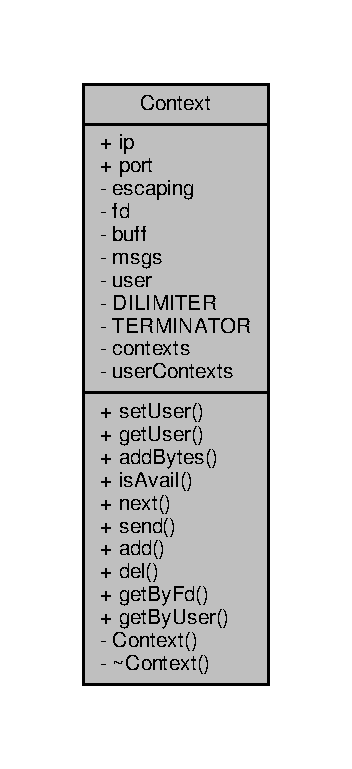
\includegraphics[width=169pt]{classContext__coll__graph}
\end{center}
\end{figure}
\subsection*{Public Member Functions}
\begin{DoxyCompactItemize}
\item 
void \hyperlink{classContext_a0c72699560699b43eef88c14e3e71943}{set\+User} (const std\+::string \&\+\_\+user)
\item 
const std\+::string \& \hyperlink{classContext_ad6a061c8ed4681e09c25eb830c29d93c}{get\+User} () const 
\item 
void \hyperlink{classContext_a124207fc0f8ef54550ae923503c487c9}{add\+Bytes} (const char $\ast$bytes, int len)
\begin{DoxyCompactList}\small\item\em Add received bytes from \hyperlink{classConn}{Conn} Protocal\+: $\vert$ Body\+: of any length $\vert$ Dilimiter $\vert$ Terminator $\vert$ Escaped text, \char`\"{}\$\$\char`\"{} for \char`\"{}\$\char`\"{} $\vert$ \char`\"{}\$\char`\"{} $\vert$ \textquotesingle{}. \end{DoxyCompactList}\item 
bool \hyperlink{classContext_a66a69e531a5f60da65bfd895756ebff9}{is\+Avail} () const 
\begin{DoxyCompactList}\small\item\em If there are available messages? \end{DoxyCompactList}\item 
std\+::string \hyperlink{classContext_a0e965560cf9a1aaba46e24bb908f49be}{next} ()
\begin{DoxyCompactList}\small\item\em Pop next message. \end{DoxyCompactList}\item 
void \hyperlink{classContext_a110781d4d93d9ffb762a34a021218877}{send} (const std\+::string \&\+\_\+msg)
\begin{DoxyCompactList}\small\item\em Send message. \end{DoxyCompactList}\end{DoxyCompactItemize}
\subsection*{Static Public Member Functions}
\begin{DoxyCompactItemize}
\item 
static void \hyperlink{classContext_a732d579c381e6bcbc3d8899c8266f4d0}{add} (int \hyperlink{classContext_aaf11c36966be14b2e1e53ee43c8e91dd}{fd}, const char $\ast$\hyperlink{classContext_a3508ad395f4b0c7e61ad46b247307f50}{ip}, unsigned short \hyperlink{classContext_a68ab96bf75c30c3497312f95ace6de91}{port})
\item 
static void \hyperlink{classContext_ab5d0194f847307302b65a387515effb8}{del} (int \hyperlink{classContext_aaf11c36966be14b2e1e53ee43c8e91dd}{fd})
\item 
static \hyperlink{classContext}{Context} \& \hyperlink{classContext_ab985f83f8262651fd9df85ba1bcb47fe}{get\+By\+Fd} (int \hyperlink{classContext_aaf11c36966be14b2e1e53ee43c8e91dd}{fd})
\item 
static const std\+::vector$<$ \hyperlink{classContext}{Context} $\ast$ $>$ \& \hyperlink{classContext_adc40dec3fe28c127523cae55097a91ce}{get\+By\+User} (const std\+::string \&name)
\end{DoxyCompactItemize}
\subsection*{Public Attributes}
\begin{DoxyCompactItemize}
\item 
const std\+::string \hyperlink{classContext_a3508ad395f4b0c7e61ad46b247307f50}{ip}
\item 
const unsigned short \hyperlink{classContext_a68ab96bf75c30c3497312f95ace6de91}{port}
\end{DoxyCompactItemize}
\subsection*{Private Member Functions}
\begin{DoxyCompactItemize}
\item 
\hyperlink{classContext_a1f8fc23ba0333d55461a81555e368162}{Context} (int \+\_\+fd, const char $\ast$\+\_\+ip, unsigned short \+\_\+port)
\item 
\hyperlink{classContext_a2d34e4556448e40693f61d15e091b604}{$\sim$\+Context} ()
\end{DoxyCompactItemize}
\subsection*{Private Attributes}
\begin{DoxyCompactItemize}
\item 
bool \hyperlink{classContext_a5f34f6e7fc17f613087021f52e2154f9}{escaping}
\item 
const int \hyperlink{classContext_aaf11c36966be14b2e1e53ee43c8e91dd}{fd}
\item 
std\+::string \hyperlink{classContext_a61817df359b6ed50d1a255648c80fd58}{buff}
\begin{DoxyCompactList}\small\item\em File descriptor. \end{DoxyCompactList}\item 
std\+::list$<$ std\+::string $>$ \hyperlink{classContext_a24115a22c1e187f610f41d9542b3516a}{msgs}
\item 
std\+::string \hyperlink{classContext_a8525c6ece0d6a53339ef8a59c1cfd668}{user}
\begin{DoxyCompactList}\small\item\em List of received messages. \end{DoxyCompactList}\end{DoxyCompactItemize}
\subsection*{Static Private Attributes}
\begin{DoxyCompactItemize}
\item 
static constexpr char \hyperlink{classContext_a63a0ff9017aba4c0d9551900093ee057}{D\+I\+L\+I\+M\+I\+T\+ER} = \textquotesingle{}\$\textquotesingle{}
\item 
static constexpr char \hyperlink{classContext_a5a12ec226a7135dc356ab34745a3f5df}{T\+E\+R\+M\+I\+N\+A\+T\+OR} = \textquotesingle{}.\textquotesingle{}
\item 
static std\+::unordered\+\_\+map$<$ int, \hyperlink{classContext}{Context} $\ast$ $>$ \hyperlink{classContext_abab3c078973688455f584747769f14fe}{contexts}
\item 
static std\+::unordered\+\_\+map$<$ std\+::string, std\+::vector$<$ \hyperlink{classContext}{Context} $\ast$ $>$ $>$ \hyperlink{classContext_a73f2f8250661a88e254e49a266f6a705}{user\+Contexts}
\end{DoxyCompactItemize}


\subsection{Detailed Description}
\hyperlink{classContext}{Context} of a connection. 

\subsection{Constructor \& Destructor Documentation}
\index{Context@{Context}!Context@{Context}}
\index{Context@{Context}!Context@{Context}}
\subsubsection[{\texorpdfstring{Context(int \+\_\+fd, const char $\ast$\+\_\+ip, unsigned short \+\_\+port)}{Context(int _fd, const char *_ip, unsigned short _port)}}]{\setlength{\rightskip}{0pt plus 5cm}Context\+::\+Context (
\begin{DoxyParamCaption}
\item[{int}]{\+\_\+fd, }
\item[{const char $\ast$}]{\+\_\+ip, }
\item[{unsigned short}]{\+\_\+port}
\end{DoxyParamCaption}
)\hspace{0.3cm}{\ttfamily [private]}}\hypertarget{classContext_a1f8fc23ba0333d55461a81555e368162}{}\label{classContext_a1f8fc23ba0333d55461a81555e368162}
\index{Context@{Context}!````~Context@{$\sim$\+Context}}
\index{````~Context@{$\sim$\+Context}!Context@{Context}}
\subsubsection[{\texorpdfstring{$\sim$\+Context()}{~Context()}}]{\setlength{\rightskip}{0pt plus 5cm}Context\+::$\sim$\+Context (
\begin{DoxyParamCaption}
{}
\end{DoxyParamCaption}
)\hspace{0.3cm}{\ttfamily [private]}}\hypertarget{classContext_a2d34e4556448e40693f61d15e091b604}{}\label{classContext_a2d34e4556448e40693f61d15e091b604}


\subsection{Member Function Documentation}
\index{Context@{Context}!add@{add}}
\index{add@{add}!Context@{Context}}
\subsubsection[{\texorpdfstring{add(int fd, const char $\ast$ip, unsigned short port)}{add(int fd, const char *ip, unsigned short port)}}]{\setlength{\rightskip}{0pt plus 5cm}void Context\+::add (
\begin{DoxyParamCaption}
\item[{int}]{fd, }
\item[{const char $\ast$}]{ip, }
\item[{unsigned short}]{port}
\end{DoxyParamCaption}
)\hspace{0.3cm}{\ttfamily [static]}}\hypertarget{classContext_a732d579c381e6bcbc3d8899c8266f4d0}{}\label{classContext_a732d579c381e6bcbc3d8899c8266f4d0}
\index{Context@{Context}!add\+Bytes@{add\+Bytes}}
\index{add\+Bytes@{add\+Bytes}!Context@{Context}}
\subsubsection[{\texorpdfstring{add\+Bytes(const char $\ast$bytes, int len)}{addBytes(const char *bytes, int len)}}]{\setlength{\rightskip}{0pt plus 5cm}void Context\+::add\+Bytes (
\begin{DoxyParamCaption}
\item[{const char $\ast$}]{bytes, }
\item[{int}]{len}
\end{DoxyParamCaption}
)}\hypertarget{classContext_a124207fc0f8ef54550ae923503c487c9}{}\label{classContext_a124207fc0f8ef54550ae923503c487c9}


Add received bytes from \hyperlink{classConn}{Conn} Protocal\+: $\vert$ Body\+: of any length $\vert$ Dilimiter $\vert$ Terminator $\vert$ Escaped text, \char`\"{}\$\$\char`\"{} for \char`\"{}\$\char`\"{} $\vert$ \char`\"{}\$\char`\"{} $\vert$ \textquotesingle{}. 

\textquotesingle{} 
\begin{DoxyExceptions}{Exceptions}
{\em } & \hyperlink{classInvalidMessage}{Invalid\+Message} \\
\hline
\end{DoxyExceptions}
\index{Context@{Context}!del@{del}}
\index{del@{del}!Context@{Context}}
\subsubsection[{\texorpdfstring{del(int fd)}{del(int fd)}}]{\setlength{\rightskip}{0pt plus 5cm}void Context\+::del (
\begin{DoxyParamCaption}
\item[{int}]{fd}
\end{DoxyParamCaption}
)\hspace{0.3cm}{\ttfamily [static]}}\hypertarget{classContext_ab5d0194f847307302b65a387515effb8}{}\label{classContext_ab5d0194f847307302b65a387515effb8}
\index{Context@{Context}!get\+By\+Fd@{get\+By\+Fd}}
\index{get\+By\+Fd@{get\+By\+Fd}!Context@{Context}}
\subsubsection[{\texorpdfstring{get\+By\+Fd(int fd)}{getByFd(int fd)}}]{\setlength{\rightskip}{0pt plus 5cm}static {\bf Context}\& Context\+::get\+By\+Fd (
\begin{DoxyParamCaption}
\item[{int}]{fd}
\end{DoxyParamCaption}
)\hspace{0.3cm}{\ttfamily [inline]}, {\ttfamily [static]}}\hypertarget{classContext_ab985f83f8262651fd9df85ba1bcb47fe}{}\label{classContext_ab985f83f8262651fd9df85ba1bcb47fe}
\index{Context@{Context}!get\+By\+User@{get\+By\+User}}
\index{get\+By\+User@{get\+By\+User}!Context@{Context}}
\subsubsection[{\texorpdfstring{get\+By\+User(const std\+::string \&name)}{getByUser(const std::string &name)}}]{\setlength{\rightskip}{0pt plus 5cm}static const std\+::vector$<${\bf Context}$\ast$$>$\& Context\+::get\+By\+User (
\begin{DoxyParamCaption}
\item[{const std\+::string \&}]{name}
\end{DoxyParamCaption}
)\hspace{0.3cm}{\ttfamily [inline]}, {\ttfamily [static]}}\hypertarget{classContext_adc40dec3fe28c127523cae55097a91ce}{}\label{classContext_adc40dec3fe28c127523cae55097a91ce}
\index{Context@{Context}!get\+User@{get\+User}}
\index{get\+User@{get\+User}!Context@{Context}}
\subsubsection[{\texorpdfstring{get\+User() const }{getUser() const }}]{\setlength{\rightskip}{0pt plus 5cm}const std\+::string\& Context\+::get\+User (
\begin{DoxyParamCaption}
{}
\end{DoxyParamCaption}
) const\hspace{0.3cm}{\ttfamily [inline]}}\hypertarget{classContext_ad6a061c8ed4681e09c25eb830c29d93c}{}\label{classContext_ad6a061c8ed4681e09c25eb830c29d93c}
\index{Context@{Context}!is\+Avail@{is\+Avail}}
\index{is\+Avail@{is\+Avail}!Context@{Context}}
\subsubsection[{\texorpdfstring{is\+Avail() const }{isAvail() const }}]{\setlength{\rightskip}{0pt plus 5cm}bool Context\+::is\+Avail (
\begin{DoxyParamCaption}
{}
\end{DoxyParamCaption}
) const\hspace{0.3cm}{\ttfamily [inline]}}\hypertarget{classContext_a66a69e531a5f60da65bfd895756ebff9}{}\label{classContext_a66a69e531a5f60da65bfd895756ebff9}


If there are available messages? 

\index{Context@{Context}!next@{next}}
\index{next@{next}!Context@{Context}}
\subsubsection[{\texorpdfstring{next()}{next()}}]{\setlength{\rightskip}{0pt plus 5cm}std\+::string Context\+::next (
\begin{DoxyParamCaption}
{}
\end{DoxyParamCaption}
)\hspace{0.3cm}{\ttfamily [inline]}}\hypertarget{classContext_a0e965560cf9a1aaba46e24bb908f49be}{}\label{classContext_a0e965560cf9a1aaba46e24bb908f49be}


Pop next message. 

\index{Context@{Context}!send@{send}}
\index{send@{send}!Context@{Context}}
\subsubsection[{\texorpdfstring{send(const std\+::string \&\+\_\+msg)}{send(const std::string &_msg)}}]{\setlength{\rightskip}{0pt plus 5cm}void Context\+::send (
\begin{DoxyParamCaption}
\item[{const std\+::string \&}]{\+\_\+msg}
\end{DoxyParamCaption}
)}\hypertarget{classContext_a110781d4d93d9ffb762a34a021218877}{}\label{classContext_a110781d4d93d9ffb762a34a021218877}


Send message. 

\index{Context@{Context}!set\+User@{set\+User}}
\index{set\+User@{set\+User}!Context@{Context}}
\subsubsection[{\texorpdfstring{set\+User(const std\+::string \&\+\_\+user)}{setUser(const std::string &_user)}}]{\setlength{\rightskip}{0pt plus 5cm}void Context\+::set\+User (
\begin{DoxyParamCaption}
\item[{const std\+::string \&}]{\+\_\+user}
\end{DoxyParamCaption}
)}\hypertarget{classContext_a0c72699560699b43eef88c14e3e71943}{}\label{classContext_a0c72699560699b43eef88c14e3e71943}


\subsection{Member Data Documentation}
\index{Context@{Context}!buff@{buff}}
\index{buff@{buff}!Context@{Context}}
\subsubsection[{\texorpdfstring{buff}{buff}}]{\setlength{\rightskip}{0pt plus 5cm}std\+::string Context\+::buff\hspace{0.3cm}{\ttfamily [private]}}\hypertarget{classContext_a61817df359b6ed50d1a255648c80fd58}{}\label{classContext_a61817df359b6ed50d1a255648c80fd58}


File descriptor. 

\index{Context@{Context}!contexts@{contexts}}
\index{contexts@{contexts}!Context@{Context}}
\subsubsection[{\texorpdfstring{contexts}{contexts}}]{\setlength{\rightskip}{0pt plus 5cm}std\+::unordered\+\_\+map$<$ int, {\bf Context} $\ast$ $>$ Context\+::contexts\hspace{0.3cm}{\ttfamily [static]}, {\ttfamily [private]}}\hypertarget{classContext_abab3c078973688455f584747769f14fe}{}\label{classContext_abab3c078973688455f584747769f14fe}
\index{Context@{Context}!D\+I\+L\+I\+M\+I\+T\+ER@{D\+I\+L\+I\+M\+I\+T\+ER}}
\index{D\+I\+L\+I\+M\+I\+T\+ER@{D\+I\+L\+I\+M\+I\+T\+ER}!Context@{Context}}
\subsubsection[{\texorpdfstring{D\+I\+L\+I\+M\+I\+T\+ER}{DILIMITER}}]{\setlength{\rightskip}{0pt plus 5cm}constexpr char Context\+::\+D\+I\+L\+I\+M\+I\+T\+ER = \textquotesingle{}\$\textquotesingle{}\hspace{0.3cm}{\ttfamily [static]}, {\ttfamily [private]}}\hypertarget{classContext_a63a0ff9017aba4c0d9551900093ee057}{}\label{classContext_a63a0ff9017aba4c0d9551900093ee057}
\index{Context@{Context}!escaping@{escaping}}
\index{escaping@{escaping}!Context@{Context}}
\subsubsection[{\texorpdfstring{escaping}{escaping}}]{\setlength{\rightskip}{0pt plus 5cm}bool Context\+::escaping\hspace{0.3cm}{\ttfamily [private]}}\hypertarget{classContext_a5f34f6e7fc17f613087021f52e2154f9}{}\label{classContext_a5f34f6e7fc17f613087021f52e2154f9}
\index{Context@{Context}!fd@{fd}}
\index{fd@{fd}!Context@{Context}}
\subsubsection[{\texorpdfstring{fd}{fd}}]{\setlength{\rightskip}{0pt plus 5cm}const int Context\+::fd\hspace{0.3cm}{\ttfamily [private]}}\hypertarget{classContext_aaf11c36966be14b2e1e53ee43c8e91dd}{}\label{classContext_aaf11c36966be14b2e1e53ee43c8e91dd}
\index{Context@{Context}!ip@{ip}}
\index{ip@{ip}!Context@{Context}}
\subsubsection[{\texorpdfstring{ip}{ip}}]{\setlength{\rightskip}{0pt plus 5cm}const std\+::string Context\+::ip}\hypertarget{classContext_a3508ad395f4b0c7e61ad46b247307f50}{}\label{classContext_a3508ad395f4b0c7e61ad46b247307f50}
\index{Context@{Context}!msgs@{msgs}}
\index{msgs@{msgs}!Context@{Context}}
\subsubsection[{\texorpdfstring{msgs}{msgs}}]{\setlength{\rightskip}{0pt plus 5cm}std\+::list$<$std\+::string$>$ Context\+::msgs\hspace{0.3cm}{\ttfamily [private]}}\hypertarget{classContext_a24115a22c1e187f610f41d9542b3516a}{}\label{classContext_a24115a22c1e187f610f41d9542b3516a}
\index{Context@{Context}!port@{port}}
\index{port@{port}!Context@{Context}}
\subsubsection[{\texorpdfstring{port}{port}}]{\setlength{\rightskip}{0pt plus 5cm}const unsigned short Context\+::port}\hypertarget{classContext_a68ab96bf75c30c3497312f95ace6de91}{}\label{classContext_a68ab96bf75c30c3497312f95ace6de91}
\index{Context@{Context}!T\+E\+R\+M\+I\+N\+A\+T\+OR@{T\+E\+R\+M\+I\+N\+A\+T\+OR}}
\index{T\+E\+R\+M\+I\+N\+A\+T\+OR@{T\+E\+R\+M\+I\+N\+A\+T\+OR}!Context@{Context}}
\subsubsection[{\texorpdfstring{T\+E\+R\+M\+I\+N\+A\+T\+OR}{TERMINATOR}}]{\setlength{\rightskip}{0pt plus 5cm}constexpr char Context\+::\+T\+E\+R\+M\+I\+N\+A\+T\+OR = \textquotesingle{}.\textquotesingle{}\hspace{0.3cm}{\ttfamily [static]}, {\ttfamily [private]}}\hypertarget{classContext_a5a12ec226a7135dc356ab34745a3f5df}{}\label{classContext_a5a12ec226a7135dc356ab34745a3f5df}
\index{Context@{Context}!user@{user}}
\index{user@{user}!Context@{Context}}
\subsubsection[{\texorpdfstring{user}{user}}]{\setlength{\rightskip}{0pt plus 5cm}std\+::string Context\+::user\hspace{0.3cm}{\ttfamily [private]}}\hypertarget{classContext_a8525c6ece0d6a53339ef8a59c1cfd668}{}\label{classContext_a8525c6ece0d6a53339ef8a59c1cfd668}


List of received messages. 

\index{Context@{Context}!user\+Contexts@{user\+Contexts}}
\index{user\+Contexts@{user\+Contexts}!Context@{Context}}
\subsubsection[{\texorpdfstring{user\+Contexts}{userContexts}}]{\setlength{\rightskip}{0pt plus 5cm}std\+::unordered\+\_\+map$<$ std\+::string, std\+::vector$<$ {\bf Context} $\ast$ $>$ $>$ Context\+::user\+Contexts\hspace{0.3cm}{\ttfamily [static]}, {\ttfamily [private]}}\hypertarget{classContext_a73f2f8250661a88e254e49a266f6a705}{}\label{classContext_a73f2f8250661a88e254e49a266f6a705}


The documentation for this class was generated from the following files\+:\begin{DoxyCompactItemize}
\item 
\hyperlink{Context_8h}{Context.\+h}\item 
\hyperlink{Context_8cpp}{Context.\+cpp}\end{DoxyCompactItemize}

\hypertarget{classInvalidMessage}{}\section{Invalid\+Message Class Reference}
\label{classInvalidMessage}\index{Invalid\+Message@{Invalid\+Message}}


{\ttfamily \#include $<$Invalid\+Message.\+h$>$}



Inheritance diagram for Invalid\+Message\+:
\nopagebreak
\begin{figure}[H]
\begin{center}
\leavevmode
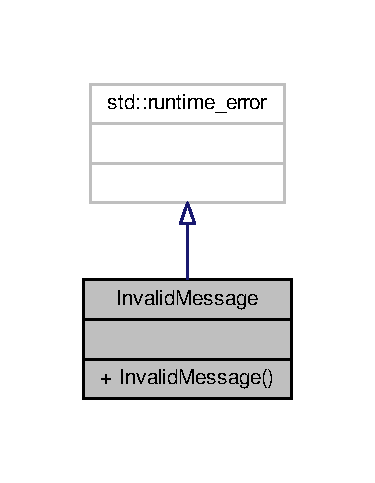
\includegraphics[width=180pt]{classInvalidMessage__inherit__graph}
\end{center}
\end{figure}


Collaboration diagram for Invalid\+Message\+:
\nopagebreak
\begin{figure}[H]
\begin{center}
\leavevmode
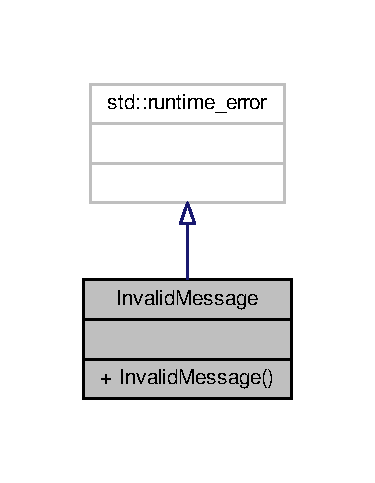
\includegraphics[width=180pt]{classInvalidMessage__coll__graph}
\end{center}
\end{figure}
\subsection*{Public Member Functions}
\begin{DoxyCompactItemize}
\item 
\hyperlink{classInvalidMessage_adf3d5539f69b1fe97910221387ad80bd}{Invalid\+Message} (const std\+::string \&what)
\end{DoxyCompactItemize}


\subsection{Constructor \& Destructor Documentation}
\index{Invalid\+Message@{Invalid\+Message}!Invalid\+Message@{Invalid\+Message}}
\index{Invalid\+Message@{Invalid\+Message}!Invalid\+Message@{Invalid\+Message}}
\subsubsection[{\texorpdfstring{Invalid\+Message(const std\+::string \&what)}{InvalidMessage(const std::string &what)}}]{\setlength{\rightskip}{0pt plus 5cm}Invalid\+Message\+::\+Invalid\+Message (
\begin{DoxyParamCaption}
\item[{const std\+::string \&}]{what}
\end{DoxyParamCaption}
)\hspace{0.3cm}{\ttfamily [inline]}}\hypertarget{classInvalidMessage_adf3d5539f69b1fe97910221387ad80bd}{}\label{classInvalidMessage_adf3d5539f69b1fe97910221387ad80bd}


The documentation for this class was generated from the following file\+:\begin{DoxyCompactItemize}
\item 
\hyperlink{InvalidMessage_8h}{Invalid\+Message.\+h}\end{DoxyCompactItemize}

\hypertarget{structMessage}{}\section{Message Struct Reference}
\label{structMessage}\index{Message@{Message}}


{\ttfamily \#include $<$Message.\+h$>$}



Collaboration diagram for Message\+:
\nopagebreak
\begin{figure}[H]
\begin{center}
\leavevmode
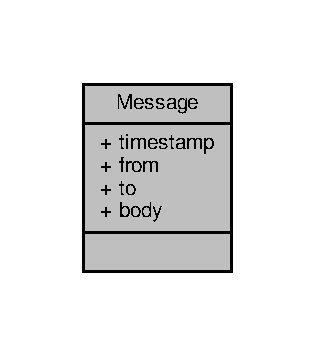
\includegraphics[width=151pt]{structMessage__coll__graph}
\end{center}
\end{figure}
\subsection*{Public Attributes}
\begin{DoxyCompactItemize}
\item 
time\+\_\+t \hyperlink{structMessage_a23d8be7ab171d014f7286587b8d1c16b}{timestamp}
\item 
std\+::string \hyperlink{structMessage_a9d1b7342dff5fedbef018e9517820263}{from}
\item 
std\+::string \hyperlink{structMessage_a094146d3f34095c1ab1395cd06c91c06}{to}
\item 
std\+::string \hyperlink{structMessage_a4e543f4898ab8a7c812caab2c21bfab7}{body}
\end{DoxyCompactItemize}


\subsection{Member Data Documentation}
\index{Message@{Message}!body@{body}}
\index{body@{body}!Message@{Message}}
\subsubsection[{\texorpdfstring{body}{body}}]{\setlength{\rightskip}{0pt plus 5cm}std\+::string Message\+::body}\hypertarget{structMessage_a4e543f4898ab8a7c812caab2c21bfab7}{}\label{structMessage_a4e543f4898ab8a7c812caab2c21bfab7}
\index{Message@{Message}!from@{from}}
\index{from@{from}!Message@{Message}}
\subsubsection[{\texorpdfstring{from}{from}}]{\setlength{\rightskip}{0pt plus 5cm}std\+::string Message\+::from}\hypertarget{structMessage_a9d1b7342dff5fedbef018e9517820263}{}\label{structMessage_a9d1b7342dff5fedbef018e9517820263}
\index{Message@{Message}!timestamp@{timestamp}}
\index{timestamp@{timestamp}!Message@{Message}}
\subsubsection[{\texorpdfstring{timestamp}{timestamp}}]{\setlength{\rightskip}{0pt plus 5cm}time\+\_\+t Message\+::timestamp}\hypertarget{structMessage_a23d8be7ab171d014f7286587b8d1c16b}{}\label{structMessage_a23d8be7ab171d014f7286587b8d1c16b}
\index{Message@{Message}!to@{to}}
\index{to@{to}!Message@{Message}}
\subsubsection[{\texorpdfstring{to}{to}}]{\setlength{\rightskip}{0pt plus 5cm}std\+::string Message\+::to}\hypertarget{structMessage_a094146d3f34095c1ab1395cd06c91c06}{}\label{structMessage_a094146d3f34095c1ab1395cd06c91c06}


The documentation for this struct was generated from the following file\+:\begin{DoxyCompactItemize}
\item 
\hyperlink{Message_8h}{Message.\+h}\end{DoxyCompactItemize}

\hypertarget{classNetworkError}{}\section{Network\+Error Class Reference}
\label{classNetworkError}\index{Network\+Error@{Network\+Error}}


{\ttfamily \#include $<$Network\+Error.\+h$>$}



Inheritance diagram for Network\+Error\+:
\nopagebreak
\begin{figure}[H]
\begin{center}
\leavevmode
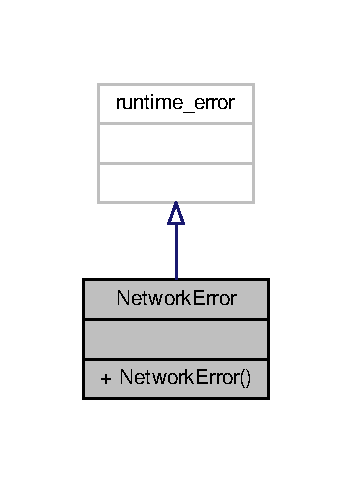
\includegraphics[width=169pt]{classNetworkError__inherit__graph}
\end{center}
\end{figure}


Collaboration diagram for Network\+Error\+:
\nopagebreak
\begin{figure}[H]
\begin{center}
\leavevmode
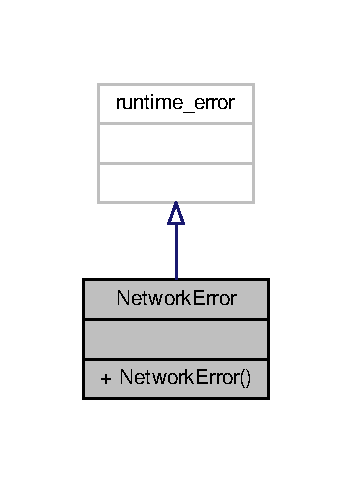
\includegraphics[width=169pt]{classNetworkError__coll__graph}
\end{center}
\end{figure}
\subsection*{Public Member Functions}
\begin{DoxyCompactItemize}
\item 
\hyperlink{classNetworkError_ae5eb4be73f9625088bbed56cf7388de3}{Network\+Error} (const std\+::string \&what)
\end{DoxyCompactItemize}


\subsection{Constructor \& Destructor Documentation}
\index{Network\+Error@{Network\+Error}!Network\+Error@{Network\+Error}}
\index{Network\+Error@{Network\+Error}!Network\+Error@{Network\+Error}}
\subsubsection[{\texorpdfstring{Network\+Error(const std\+::string \&what)}{NetworkError(const std::string &what)}}]{\setlength{\rightskip}{0pt plus 5cm}Network\+Error\+::\+Network\+Error (
\begin{DoxyParamCaption}
\item[{const std\+::string \&}]{what}
\end{DoxyParamCaption}
)\hspace{0.3cm}{\ttfamily [inline]}}\hypertarget{classNetworkError_ae5eb4be73f9625088bbed56cf7388de3}{}\label{classNetworkError_ae5eb4be73f9625088bbed56cf7388de3}


The documentation for this class was generated from the following file\+:\begin{DoxyCompactItemize}
\item 
\hyperlink{NetworkError_8h}{Network\+Error.\+h}\end{DoxyCompactItemize}

\hypertarget{structUser}{}\section{User Struct Reference}
\label{structUser}\index{User@{User}}


{\ttfamily \#include $<$User.\+h$>$}



Collaboration diagram for User\+:
\nopagebreak
\begin{figure}[H]
\begin{center}
\leavevmode
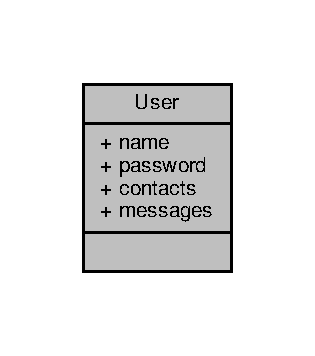
\includegraphics[width=151pt]{structUser__coll__graph}
\end{center}
\end{figure}
\subsection*{Public Attributes}
\begin{DoxyCompactItemize}
\item 
std\+::string \hyperlink{structUser_a085d8d69282b6298964eab8351584536}{name}
\item 
std\+::string \hyperlink{structUser_ac2f2e75b15e8eb6cbb030fc85a6cd59f}{password}
\item 
std\+::vector$<$ std\+::string $>$ \hyperlink{structUser_ab020b301809cbced04dd78f324fa3e2e}{contacts}
\item 
std\+::vector$<$ int $>$ \hyperlink{structUser_a1b194a13658a19f18233e0d5b102e295}{messages}
\end{DoxyCompactItemize}


\subsection{Member Data Documentation}
\index{User@{User}!contacts@{contacts}}
\index{contacts@{contacts}!User@{User}}
\subsubsection[{\texorpdfstring{contacts}{contacts}}]{\setlength{\rightskip}{0pt plus 5cm}std\+::vector$<$std\+::string$>$ User\+::contacts}\hypertarget{structUser_ab020b301809cbced04dd78f324fa3e2e}{}\label{structUser_ab020b301809cbced04dd78f324fa3e2e}
\index{User@{User}!messages@{messages}}
\index{messages@{messages}!User@{User}}
\subsubsection[{\texorpdfstring{messages}{messages}}]{\setlength{\rightskip}{0pt plus 5cm}std\+::vector$<$int$>$ User\+::messages}\hypertarget{structUser_a1b194a13658a19f18233e0d5b102e295}{}\label{structUser_a1b194a13658a19f18233e0d5b102e295}
\index{User@{User}!name@{name}}
\index{name@{name}!User@{User}}
\subsubsection[{\texorpdfstring{name}{name}}]{\setlength{\rightskip}{0pt plus 5cm}std\+::string User\+::name}\hypertarget{structUser_a085d8d69282b6298964eab8351584536}{}\label{structUser_a085d8d69282b6298964eab8351584536}
\index{User@{User}!password@{password}}
\index{password@{password}!User@{User}}
\subsubsection[{\texorpdfstring{password}{password}}]{\setlength{\rightskip}{0pt plus 5cm}std\+::string User\+::password}\hypertarget{structUser_ac2f2e75b15e8eb6cbb030fc85a6cd59f}{}\label{structUser_ac2f2e75b15e8eb6cbb030fc85a6cd59f}


The documentation for this struct was generated from the following file\+:\begin{DoxyCompactItemize}
\item 
\hyperlink{User_8h}{User.\+h}\end{DoxyCompactItemize}

\chapter{File Documentation}
\hypertarget{CmdFailed_8h}{}\section{Cmd\+Failed.\+h File Reference}
\label{CmdFailed_8h}\index{Cmd\+Failed.\+h@{Cmd\+Failed.\+h}}
{\ttfamily \#include $<$string$>$}\\*
{\ttfamily \#include $<$stdexcept$>$}\\*
Include dependency graph for Cmd\+Failed.\+h\+:
\nopagebreak
\begin{figure}[H]
\begin{center}
\leavevmode
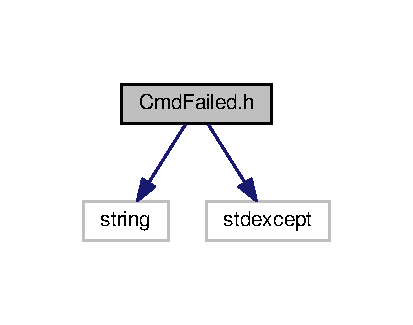
\includegraphics[width=198pt]{CmdFailed_8h__incl}
\end{center}
\end{figure}
This graph shows which files directly or indirectly include this file\+:
\nopagebreak
\begin{figure}[H]
\begin{center}
\leavevmode
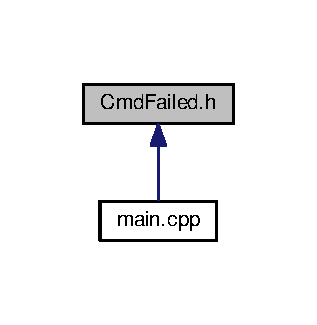
\includegraphics[width=152pt]{CmdFailed_8h__dep__incl}
\end{center}
\end{figure}
\subsection*{Classes}
\begin{DoxyCompactItemize}
\item 
class \hyperlink{classCmdFailed}{Cmd\+Failed}
\end{DoxyCompactItemize}

\hypertarget{config_8h}{}\section{config.\+h File Reference}
\label{config_8h}\index{config.\+h@{config.\+h}}
This graph shows which files directly or indirectly include this file\+:
\nopagebreak
\begin{figure}[H]
\begin{center}
\leavevmode
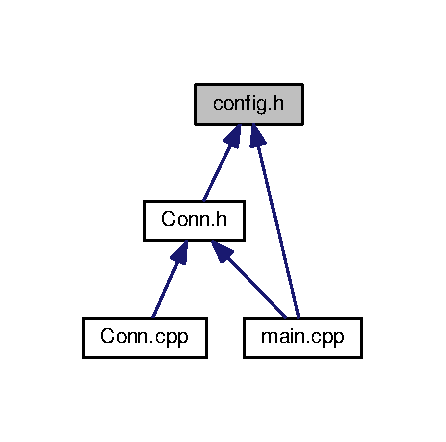
\includegraphics[width=214pt]{config_8h__dep__incl}
\end{center}
\end{figure}
\subsection*{Variables}
\begin{DoxyCompactItemize}
\item 
const unsigned short \hyperlink{config_8h_a732dec0ff237041537a9b46a40de8a59}{P\+O\+RT} = 19623
\begin{DoxyCompactList}\small\item\em T\+CP port. \end{DoxyCompactList}\item 
const int \hyperlink{config_8h_a7549d09c5c82a73df378d4919e4fd2cc}{M\+A\+X\+\_\+\+P\+E\+N\+D\+I\+N\+G\+\_\+\+C\+O\+NN} = 64
\begin{DoxyCompactList}\small\item\em Max \# of connections wait to be accepted. \end{DoxyCompactList}\item 
const int \hyperlink{config_8h_a96f3a9710263a8c7fe010108a990c28e}{D\+E\+F\+A\+U\+L\+T\+\_\+\+E\+P\+O\+L\+L\+\_\+\+P\+O\+OL} = 512
\begin{DoxyCompactList}\small\item\em Default pool size of epoll. \end{DoxyCompactList}\item 
const int \hyperlink{config_8h_abc13b0576e197f933513df9ba2ea93b6}{E\+P\+O\+L\+L\+\_\+\+N\+U\+M\+\_\+\+O\+N\+E\+\_\+\+W\+A\+IT} = 16
\begin{DoxyCompactList}\small\item\em Max \# of connections handled after one wait for epoll. \end{DoxyCompactList}\item 
const int \hyperlink{config_8h_ae1a3492267f3f3b4eab07eb800197dad}{M\+S\+G\+\_\+\+B\+U\+F\+\_\+\+S\+I\+ZE} = 1024
\begin{DoxyCompactList}\small\item\em Size of message buffer used to send or receive. \end{DoxyCompactList}\item 
const int \hyperlink{config_8h_a389b7ba5f2745b53d7d32cb30230c8ef}{M\+A\+X\+\_\+\+L\+O\+G\+\_\+\+N\+UM} = 128
\begin{DoxyCompactList}\small\item\em Max \# of logs returned once. \end{DoxyCompactList}\end{DoxyCompactItemize}


\subsection{Variable Documentation}
\index{config.\+h@{config.\+h}!D\+E\+F\+A\+U\+L\+T\+\_\+\+E\+P\+O\+L\+L\+\_\+\+P\+O\+OL@{D\+E\+F\+A\+U\+L\+T\+\_\+\+E\+P\+O\+L\+L\+\_\+\+P\+O\+OL}}
\index{D\+E\+F\+A\+U\+L\+T\+\_\+\+E\+P\+O\+L\+L\+\_\+\+P\+O\+OL@{D\+E\+F\+A\+U\+L\+T\+\_\+\+E\+P\+O\+L\+L\+\_\+\+P\+O\+OL}!config.\+h@{config.\+h}}
\subsubsection[{\texorpdfstring{D\+E\+F\+A\+U\+L\+T\+\_\+\+E\+P\+O\+L\+L\+\_\+\+P\+O\+OL}{DEFAULT_EPOLL_POOL}}]{\setlength{\rightskip}{0pt plus 5cm}const int D\+E\+F\+A\+U\+L\+T\+\_\+\+E\+P\+O\+L\+L\+\_\+\+P\+O\+OL = 512}\hypertarget{config_8h_a96f3a9710263a8c7fe010108a990c28e}{}\label{config_8h_a96f3a9710263a8c7fe010108a990c28e}


Default pool size of epoll. 

\index{config.\+h@{config.\+h}!E\+P\+O\+L\+L\+\_\+\+N\+U\+M\+\_\+\+O\+N\+E\+\_\+\+W\+A\+IT@{E\+P\+O\+L\+L\+\_\+\+N\+U\+M\+\_\+\+O\+N\+E\+\_\+\+W\+A\+IT}}
\index{E\+P\+O\+L\+L\+\_\+\+N\+U\+M\+\_\+\+O\+N\+E\+\_\+\+W\+A\+IT@{E\+P\+O\+L\+L\+\_\+\+N\+U\+M\+\_\+\+O\+N\+E\+\_\+\+W\+A\+IT}!config.\+h@{config.\+h}}
\subsubsection[{\texorpdfstring{E\+P\+O\+L\+L\+\_\+\+N\+U\+M\+\_\+\+O\+N\+E\+\_\+\+W\+A\+IT}{EPOLL_NUM_ONE_WAIT}}]{\setlength{\rightskip}{0pt plus 5cm}const int E\+P\+O\+L\+L\+\_\+\+N\+U\+M\+\_\+\+O\+N\+E\+\_\+\+W\+A\+IT = 16}\hypertarget{config_8h_abc13b0576e197f933513df9ba2ea93b6}{}\label{config_8h_abc13b0576e197f933513df9ba2ea93b6}


Max \# of connections handled after one wait for epoll. 

\index{config.\+h@{config.\+h}!M\+A\+X\+\_\+\+L\+O\+G\+\_\+\+N\+UM@{M\+A\+X\+\_\+\+L\+O\+G\+\_\+\+N\+UM}}
\index{M\+A\+X\+\_\+\+L\+O\+G\+\_\+\+N\+UM@{M\+A\+X\+\_\+\+L\+O\+G\+\_\+\+N\+UM}!config.\+h@{config.\+h}}
\subsubsection[{\texorpdfstring{M\+A\+X\+\_\+\+L\+O\+G\+\_\+\+N\+UM}{MAX_LOG_NUM}}]{\setlength{\rightskip}{0pt plus 5cm}const int M\+A\+X\+\_\+\+L\+O\+G\+\_\+\+N\+UM = 128}\hypertarget{config_8h_a389b7ba5f2745b53d7d32cb30230c8ef}{}\label{config_8h_a389b7ba5f2745b53d7d32cb30230c8ef}


Max \# of logs returned once. 

\index{config.\+h@{config.\+h}!M\+A\+X\+\_\+\+P\+E\+N\+D\+I\+N\+G\+\_\+\+C\+O\+NN@{M\+A\+X\+\_\+\+P\+E\+N\+D\+I\+N\+G\+\_\+\+C\+O\+NN}}
\index{M\+A\+X\+\_\+\+P\+E\+N\+D\+I\+N\+G\+\_\+\+C\+O\+NN@{M\+A\+X\+\_\+\+P\+E\+N\+D\+I\+N\+G\+\_\+\+C\+O\+NN}!config.\+h@{config.\+h}}
\subsubsection[{\texorpdfstring{M\+A\+X\+\_\+\+P\+E\+N\+D\+I\+N\+G\+\_\+\+C\+O\+NN}{MAX_PENDING_CONN}}]{\setlength{\rightskip}{0pt plus 5cm}const int M\+A\+X\+\_\+\+P\+E\+N\+D\+I\+N\+G\+\_\+\+C\+O\+NN = 64}\hypertarget{config_8h_a7549d09c5c82a73df378d4919e4fd2cc}{}\label{config_8h_a7549d09c5c82a73df378d4919e4fd2cc}


Max \# of connections wait to be accepted. 

\index{config.\+h@{config.\+h}!M\+S\+G\+\_\+\+B\+U\+F\+\_\+\+S\+I\+ZE@{M\+S\+G\+\_\+\+B\+U\+F\+\_\+\+S\+I\+ZE}}
\index{M\+S\+G\+\_\+\+B\+U\+F\+\_\+\+S\+I\+ZE@{M\+S\+G\+\_\+\+B\+U\+F\+\_\+\+S\+I\+ZE}!config.\+h@{config.\+h}}
\subsubsection[{\texorpdfstring{M\+S\+G\+\_\+\+B\+U\+F\+\_\+\+S\+I\+ZE}{MSG_BUF_SIZE}}]{\setlength{\rightskip}{0pt plus 5cm}const int M\+S\+G\+\_\+\+B\+U\+F\+\_\+\+S\+I\+ZE = 1024}\hypertarget{config_8h_ae1a3492267f3f3b4eab07eb800197dad}{}\label{config_8h_ae1a3492267f3f3b4eab07eb800197dad}


Size of message buffer used to send or receive. 

\index{config.\+h@{config.\+h}!P\+O\+RT@{P\+O\+RT}}
\index{P\+O\+RT@{P\+O\+RT}!config.\+h@{config.\+h}}
\subsubsection[{\texorpdfstring{P\+O\+RT}{PORT}}]{\setlength{\rightskip}{0pt plus 5cm}const unsigned short P\+O\+RT = 19623}\hypertarget{config_8h_a732dec0ff237041537a9b46a40de8a59}{}\label{config_8h_a732dec0ff237041537a9b46a40de8a59}


T\+CP port. 


\hypertarget{Conn_8cpp}{}\section{Conn.\+cpp File Reference}
\label{Conn_8cpp}\index{Conn.\+cpp@{Conn.\+cpp}}
{\ttfamily \#include $<$iostream$>$}\\*
{\ttfamily \#include \char`\"{}Conn.\+h\char`\"{}}\\*
Include dependency graph for Conn.\+cpp\+:
\nopagebreak
\begin{figure}[H]
\begin{center}
\leavevmode
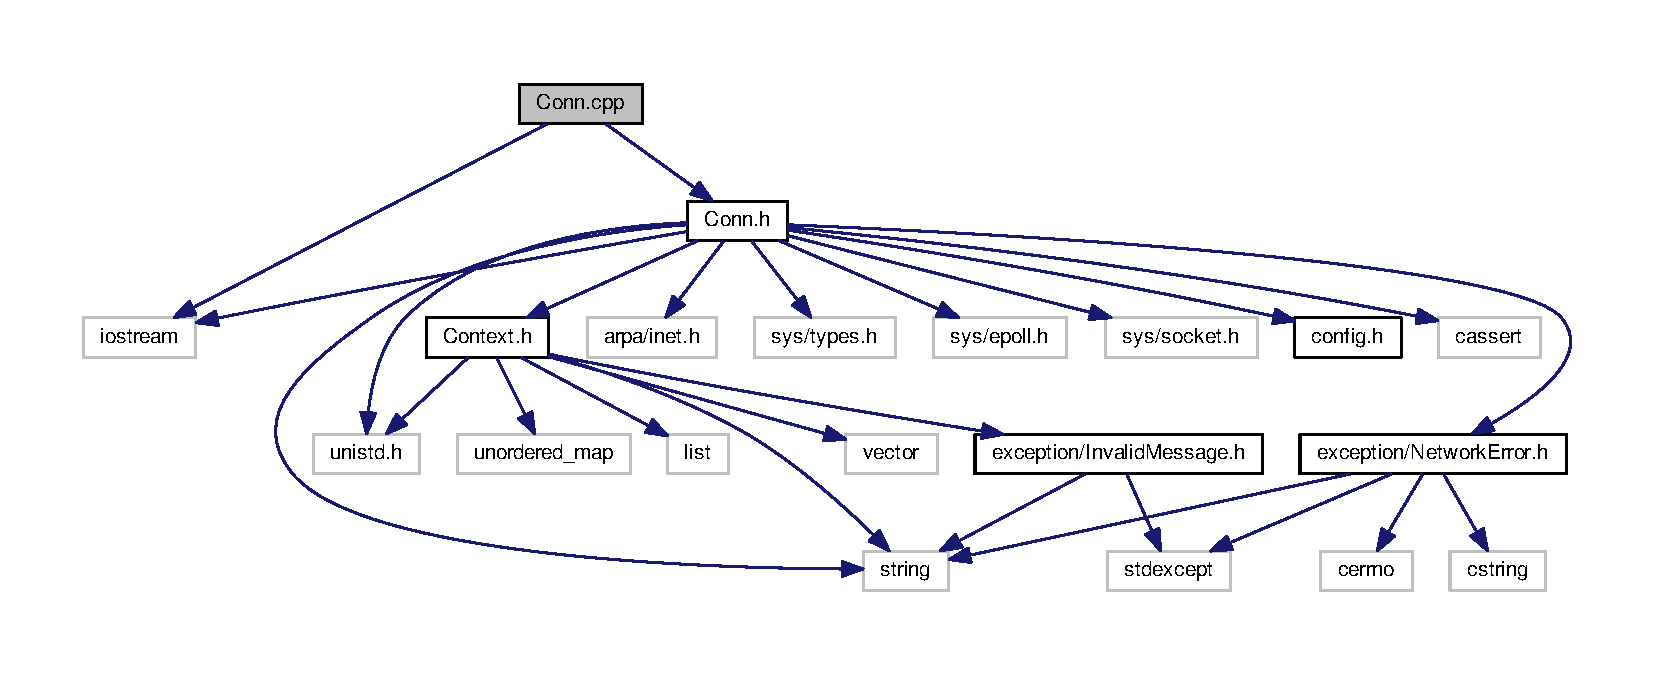
\includegraphics[width=350pt]{Conn_8cpp__incl}
\end{center}
\end{figure}

\hypertarget{Conn_8h}{}\section{Conn.\+h File Reference}
\label{Conn_8h}\index{Conn.\+h@{Conn.\+h}}
{\ttfamily \#include $<$cassert$>$}\\*
{\ttfamily \#include $<$string$>$}\\*
{\ttfamily \#include $<$iostream$>$}\\*
{\ttfamily \#include $<$unistd.\+h$>$}\\*
{\ttfamily \#include $<$arpa/inet.\+h$>$}\\*
{\ttfamily \#include $<$sys/types.\+h$>$}\\*
{\ttfamily \#include $<$sys/epoll.\+h$>$}\\*
{\ttfamily \#include $<$sys/socket.\+h$>$}\\*
{\ttfamily \#include \char`\"{}config.\+h\char`\"{}}\\*
{\ttfamily \#include \char`\"{}Context.\+h\char`\"{}}\\*
{\ttfamily \#include \char`\"{}exception/\+Network\+Error.\+h\char`\"{}}\\*
Include dependency graph for Conn.\+h\+:
\nopagebreak
\begin{figure}[H]
\begin{center}
\leavevmode
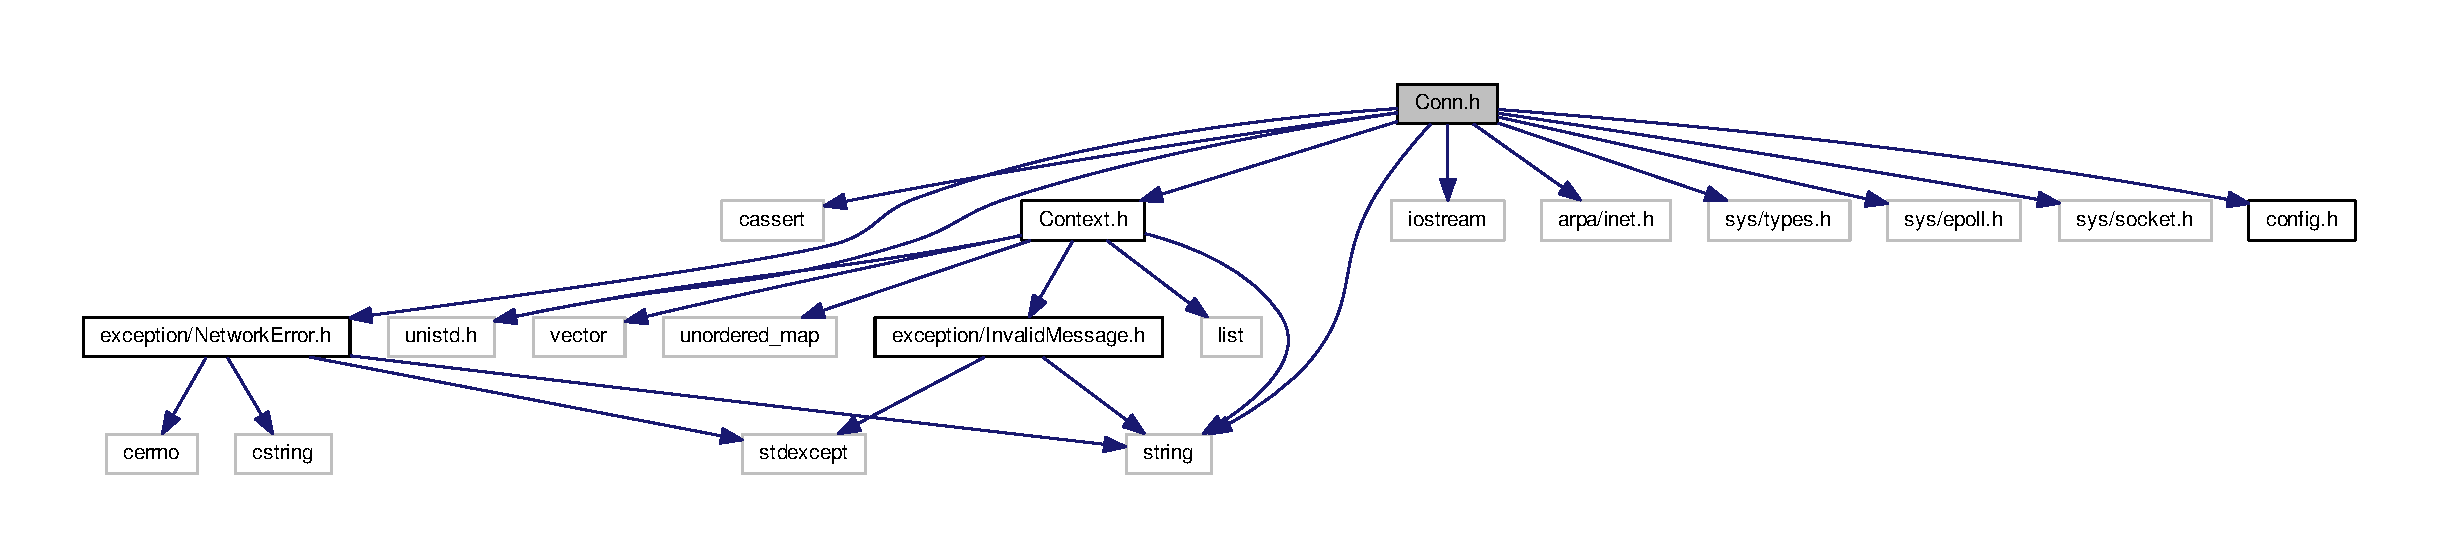
\includegraphics[width=350pt]{Conn_8h__incl}
\end{center}
\end{figure}
This graph shows which files directly or indirectly include this file\+:
\nopagebreak
\begin{figure}[H]
\begin{center}
\leavevmode
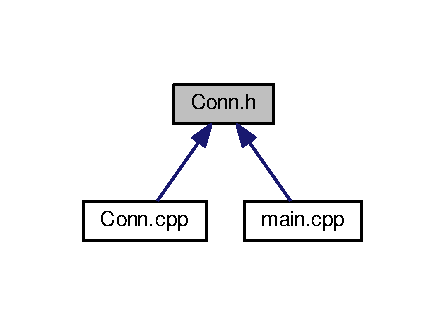
\includegraphics[width=214pt]{Conn_8h__dep__incl}
\end{center}
\end{figure}
\subsection*{Classes}
\begin{DoxyCompactItemize}
\item 
class \hyperlink{classConn}{Conn}
\begin{DoxyCompactList}\small\item\em Connection manager. \end{DoxyCompactList}\end{DoxyCompactItemize}

\hypertarget{Context_8cpp}{}\section{Context.\+cpp File Reference}
\label{Context_8cpp}\index{Context.\+cpp@{Context.\+cpp}}
{\ttfamily \#include $<$iostream$>$}\\*
{\ttfamily \#include $<$algorithm$>$}\\*
{\ttfamily \#include $<$unistd.\+h$>$}\\*
{\ttfamily \#include \char`\"{}Context.\+h\char`\"{}}\\*
Include dependency graph for Context.\+cpp\+:
\nopagebreak
\begin{figure}[H]
\begin{center}
\leavevmode
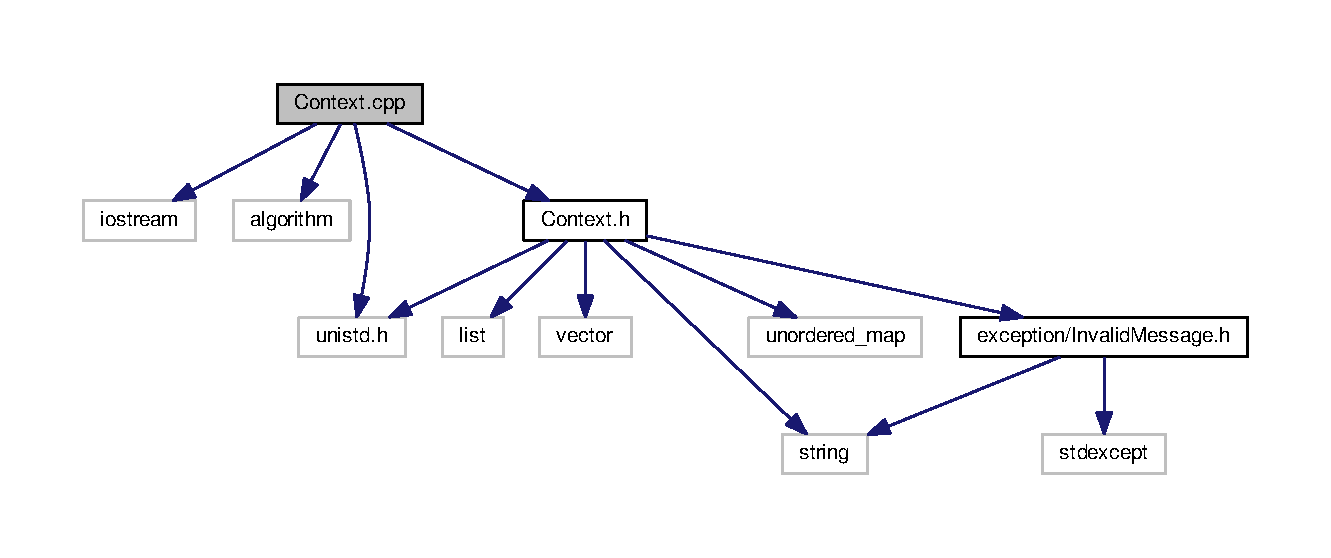
\includegraphics[width=350pt]{Context_8cpp__incl}
\end{center}
\end{figure}

\hypertarget{Context_8h}{}\section{Context.\+h File Reference}
\label{Context_8h}\index{Context.\+h@{Context.\+h}}
{\ttfamily \#include $<$list$>$}\\*
{\ttfamily \#include $<$vector$>$}\\*
{\ttfamily \#include $<$string$>$}\\*
{\ttfamily \#include $<$unordered\+\_\+map$>$}\\*
{\ttfamily \#include $<$unistd.\+h$>$}\\*
{\ttfamily \#include \char`\"{}exception/\+Invalid\+Message.\+h\char`\"{}}\\*
Include dependency graph for Context.\+h\+:
\nopagebreak
\begin{figure}[H]
\begin{center}
\leavevmode
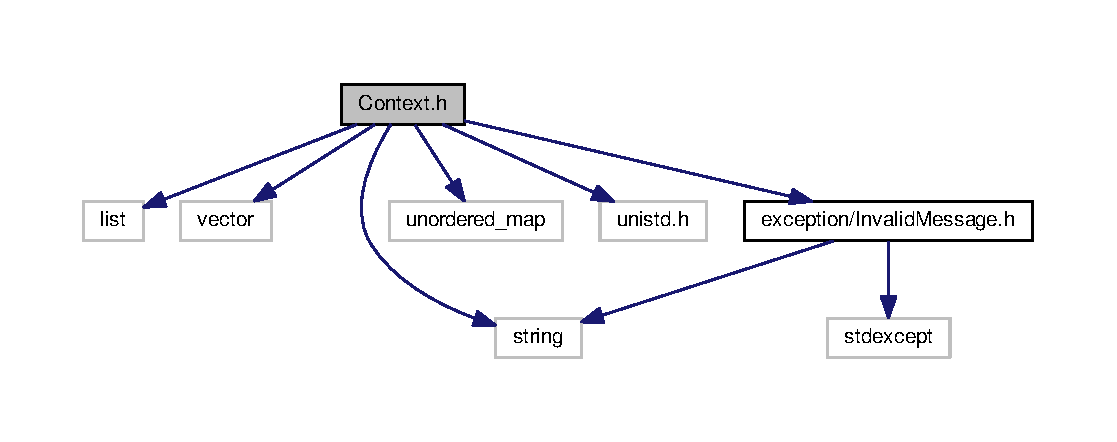
\includegraphics[width=350pt]{Context_8h__incl}
\end{center}
\end{figure}
This graph shows which files directly or indirectly include this file\+:
\nopagebreak
\begin{figure}[H]
\begin{center}
\leavevmode
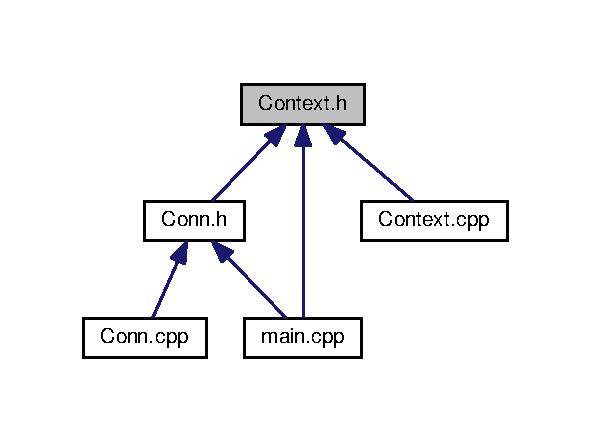
\includegraphics[width=284pt]{Context_8h__dep__incl}
\end{center}
\end{figure}
\subsection*{Classes}
\begin{DoxyCompactItemize}
\item 
class \hyperlink{classContext}{Context}
\begin{DoxyCompactList}\small\item\em \hyperlink{classContext}{Context} of a connection. \end{DoxyCompactList}\end{DoxyCompactItemize}

\hypertarget{InvalidMessage_8h}{}\section{Invalid\+Message.\+h File Reference}
\label{InvalidMessage_8h}\index{Invalid\+Message.\+h@{Invalid\+Message.\+h}}
{\ttfamily \#include $<$string$>$}\\*
{\ttfamily \#include $<$stdexcept$>$}\\*
Include dependency graph for Invalid\+Message.\+h\+:
\nopagebreak
\begin{figure}[H]
\begin{center}
\leavevmode
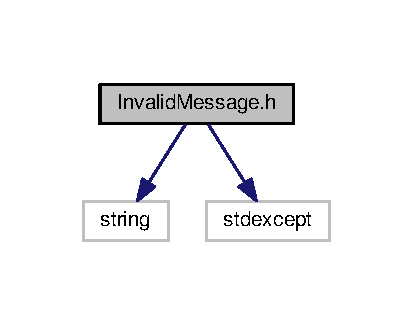
\includegraphics[width=198pt]{InvalidMessage_8h__incl}
\end{center}
\end{figure}
This graph shows which files directly or indirectly include this file\+:
\nopagebreak
\begin{figure}[H]
\begin{center}
\leavevmode
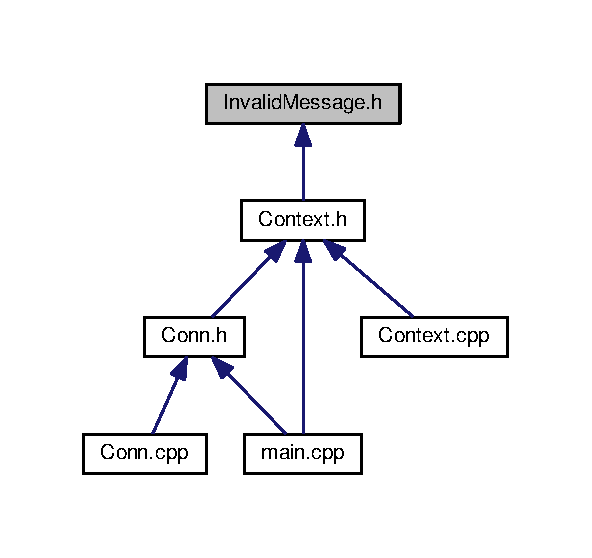
\includegraphics[width=284pt]{InvalidMessage_8h__dep__incl}
\end{center}
\end{figure}
\subsection*{Classes}
\begin{DoxyCompactItemize}
\item 
class \hyperlink{classInvalidMessage}{Invalid\+Message}
\end{DoxyCompactItemize}

\hypertarget{main_8cpp}{}\section{main.\+cpp File Reference}
\label{main_8cpp}\index{main.\+cpp@{main.\+cpp}}
{\ttfamily \#include $<$ctime$>$}\\*
{\ttfamily \#include $<$vector$>$}\\*
{\ttfamily \#include $<$iostream$>$}\\*
{\ttfamily \#include $<$algorithm$>$}\\*
{\ttfamily \#include $<$unordered\+\_\+map$>$}\\*
{\ttfamily \#include \char`\"{}User.\+h\char`\"{}}\\*
{\ttfamily \#include \char`\"{}Conn.\+h\char`\"{}}\\*
{\ttfamily \#include \char`\"{}config.\+h\char`\"{}}\\*
{\ttfamily \#include \char`\"{}Context.\+h\char`\"{}}\\*
{\ttfamily \#include \char`\"{}Message.\+h\char`\"{}}\\*
{\ttfamily \#include \char`\"{}3rd-\/party/json.\+hpp\char`\"{}}\\*
{\ttfamily \#include \char`\"{}exception/\+Cmd\+Failed.\+h\char`\"{}}\\*
Include dependency graph for main.\+cpp\+:
\nopagebreak
\begin{figure}[H]
\begin{center}
\leavevmode
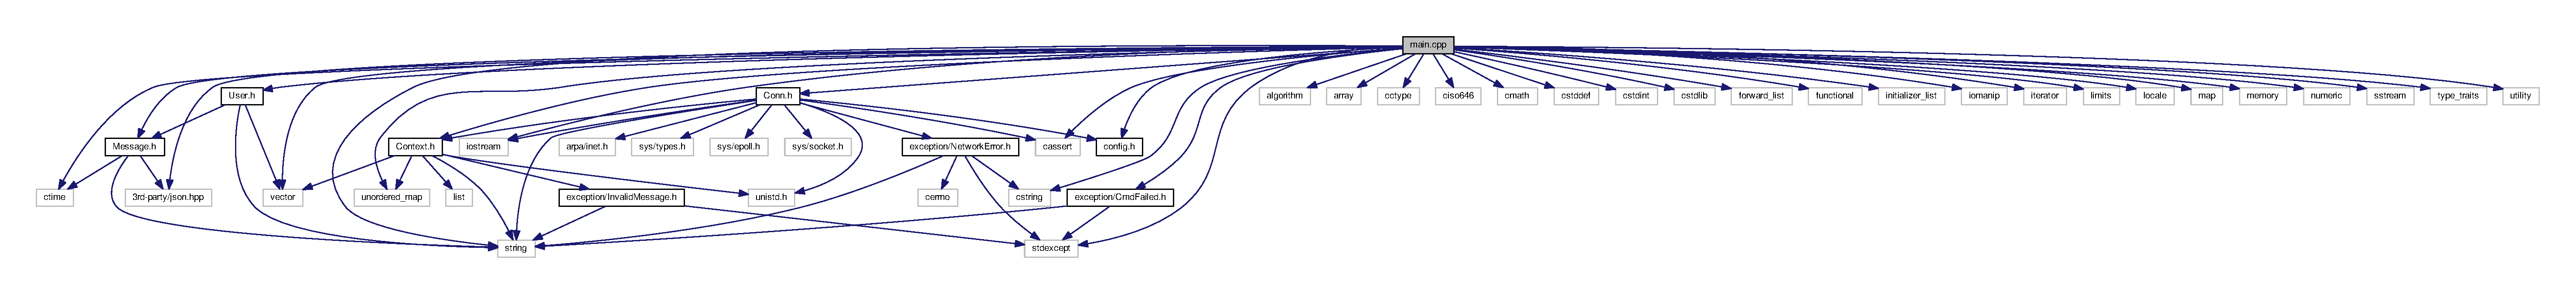
\includegraphics[width=350pt]{main_8cpp__incl}
\end{center}
\end{figure}
\subsection*{Typedefs}
\begin{DoxyCompactItemize}
\item 
using \hyperlink{main_8cpp_af13a1979f9e8f62c101433fac6511cc6}{Json} = nlohmann\+::json
\end{DoxyCompactItemize}
\subsection*{Functions}
\begin{DoxyCompactItemize}
\item 
void \hyperlink{main_8cpp_ac8aa0cf225f36a1eb1139ff06036c725}{sign\+Up} (const std\+::string \&name, const std\+::string \&password)
\begin{DoxyCompactList}\small\item\em Try to register (\char`\"{}register\char`\"{} is a C++ keyword) \end{DoxyCompactList}\item 
void \hyperlink{main_8cpp_ac9db97369440a3088ab249e3d80201e9}{login} (const std\+::string \&name, const std\+::string \&password)
\begin{DoxyCompactList}\small\item\em Try to login. \end{DoxyCompactList}\item 
std\+::vector$<$ \hyperlink{structMessage}{Message} $>$ \hyperlink{main_8cpp_a8e27fd6ddf3965828c2c8c8a8a4b7233}{get\+Log\+Since} (const std\+::string \&name, time\+\_\+t since)
\begin{DoxyCompactList}\small\item\em Get messages since a timestamp. \end{DoxyCompactList}\item 
const std\+::vector$<$ std\+::string $>$ \& \hyperlink{main_8cpp_a5866776cea9a1acfa23285185e91dd34}{upd\+Contact} (const std\+::string \&my\+Name, const std\+::string \&op, const std\+::string \&name)
\begin{DoxyCompactList}\small\item\em Update contacts of user {\ttfamily my\+Name} \end{DoxyCompactList}\item 
int \hyperlink{main_8cpp_ae66f6b31b5ad750f1fe042a706a4e3d4}{main} ()
\end{DoxyCompactItemize}
\subsection*{Variables}
\begin{DoxyCompactItemize}
\item 
std\+::unordered\+\_\+map$<$ std\+::string, \hyperlink{structUser}{User} $>$ \hyperlink{main_8cpp_aa46ebcccaa00a5a83a513bc0e2edb1e2}{users}
\item 
std\+::unordered\+\_\+map$<$ std\+::string, std\+::string $>$ \hyperlink{main_8cpp_a551b85ea30a9afeb6c88cfb58ecb3b29}{profiles}
\item 
std\+::vector$<$ \hyperlink{structMessage}{Message} $>$ \hyperlink{main_8cpp_a80da17149a00a414bb75d88c22998255}{messages}
\end{DoxyCompactItemize}


\subsection{Typedef Documentation}
\index{main.\+cpp@{main.\+cpp}!Json@{Json}}
\index{Json@{Json}!main.\+cpp@{main.\+cpp}}
\subsubsection[{\texorpdfstring{Json}{Json}}]{\setlength{\rightskip}{0pt plus 5cm}using {\bf Json} =  nlohmann\+::json}\hypertarget{main_8cpp_af13a1979f9e8f62c101433fac6511cc6}{}\label{main_8cpp_af13a1979f9e8f62c101433fac6511cc6}


\subsection{Function Documentation}
\index{main.\+cpp@{main.\+cpp}!get\+Log\+Since@{get\+Log\+Since}}
\index{get\+Log\+Since@{get\+Log\+Since}!main.\+cpp@{main.\+cpp}}
\subsubsection[{\texorpdfstring{get\+Log\+Since(const std\+::string \&name, time\+\_\+t since)}{getLogSince(const std::string &name, time_t since)}}]{\setlength{\rightskip}{0pt plus 5cm}std\+::vector$<${\bf Message}$>$ get\+Log\+Since (
\begin{DoxyParamCaption}
\item[{const std\+::string \&}]{name, }
\item[{time\+\_\+t}]{since}
\end{DoxyParamCaption}
)}\hypertarget{main_8cpp_a8e27fd6ddf3965828c2c8c8a8a4b7233}{}\label{main_8cpp_a8e27fd6ddf3965828c2c8c8a8a4b7233}


Get messages since a timestamp. 

\begin{DoxyReturn}{Returns}
M\+A\+X\+\_\+\+L\+O\+G\+\_\+\+N\+UM logs at maximum, except that there are same timestamps 
\end{DoxyReturn}
\index{main.\+cpp@{main.\+cpp}!login@{login}}
\index{login@{login}!main.\+cpp@{main.\+cpp}}
\subsubsection[{\texorpdfstring{login(const std\+::string \&name, const std\+::string \&password)}{login(const std::string &name, const std::string &password)}}]{\setlength{\rightskip}{0pt plus 5cm}void login (
\begin{DoxyParamCaption}
\item[{const std\+::string \&}]{name, }
\item[{const std\+::string \&}]{password}
\end{DoxyParamCaption}
)}\hypertarget{main_8cpp_ac9db97369440a3088ab249e3d80201e9}{}\label{main_8cpp_ac9db97369440a3088ab249e3d80201e9}


Try to login. 


\begin{DoxyExceptions}{Exceptions}
{\em } & \hyperlink{classCmdFailed}{Cmd\+Failed} \\
\hline
\end{DoxyExceptions}
\index{main.\+cpp@{main.\+cpp}!main@{main}}
\index{main@{main}!main.\+cpp@{main.\+cpp}}
\subsubsection[{\texorpdfstring{main()}{main()}}]{\setlength{\rightskip}{0pt plus 5cm}int main (
\begin{DoxyParamCaption}
{}
\end{DoxyParamCaption}
)}\hypertarget{main_8cpp_ae66f6b31b5ad750f1fe042a706a4e3d4}{}\label{main_8cpp_ae66f6b31b5ad750f1fe042a706a4e3d4}
\index{main.\+cpp@{main.\+cpp}!sign\+Up@{sign\+Up}}
\index{sign\+Up@{sign\+Up}!main.\+cpp@{main.\+cpp}}
\subsubsection[{\texorpdfstring{sign\+Up(const std\+::string \&name, const std\+::string \&password)}{signUp(const std::string &name, const std::string &password)}}]{\setlength{\rightskip}{0pt plus 5cm}void sign\+Up (
\begin{DoxyParamCaption}
\item[{const std\+::string \&}]{name, }
\item[{const std\+::string \&}]{password}
\end{DoxyParamCaption}
)}\hypertarget{main_8cpp_ac8aa0cf225f36a1eb1139ff06036c725}{}\label{main_8cpp_ac8aa0cf225f36a1eb1139ff06036c725}


Try to register (\char`\"{}register\char`\"{} is a C++ keyword) 


\begin{DoxyExceptions}{Exceptions}
{\em } & \hyperlink{classCmdFailed}{Cmd\+Failed} \\
\hline
\end{DoxyExceptions}
\index{main.\+cpp@{main.\+cpp}!upd\+Contact@{upd\+Contact}}
\index{upd\+Contact@{upd\+Contact}!main.\+cpp@{main.\+cpp}}
\subsubsection[{\texorpdfstring{upd\+Contact(const std\+::string \&my\+Name, const std\+::string \&op, const std\+::string \&name)}{updContact(const std::string &myName, const std::string &op, const std::string &name)}}]{\setlength{\rightskip}{0pt plus 5cm}const std\+::vector$<$std\+::string$>$\& upd\+Contact (
\begin{DoxyParamCaption}
\item[{const std\+::string \&}]{my\+Name, }
\item[{const std\+::string \&}]{op, }
\item[{const std\+::string \&}]{name}
\end{DoxyParamCaption}
)}\hypertarget{main_8cpp_a5866776cea9a1acfa23285185e91dd34}{}\label{main_8cpp_a5866776cea9a1acfa23285185e91dd34}


Update contacts of user {\ttfamily my\+Name} 


\begin{DoxyParams}{Parameters}
{\em op} & \+: \char`\"{}add\char`\"{} or \char`\"{}del\char`\"{} \\
\hline
\end{DoxyParams}
\begin{DoxyReturn}{Returns}
\+: Updated contacts 
\end{DoxyReturn}


\subsection{Variable Documentation}
\index{main.\+cpp@{main.\+cpp}!messages@{messages}}
\index{messages@{messages}!main.\+cpp@{main.\+cpp}}
\subsubsection[{\texorpdfstring{messages}{messages}}]{\setlength{\rightskip}{0pt plus 5cm}std\+::vector$<${\bf Message}$>$ messages}\hypertarget{main_8cpp_a80da17149a00a414bb75d88c22998255}{}\label{main_8cpp_a80da17149a00a414bb75d88c22998255}
\index{main.\+cpp@{main.\+cpp}!profiles@{profiles}}
\index{profiles@{profiles}!main.\+cpp@{main.\+cpp}}
\subsubsection[{\texorpdfstring{profiles}{profiles}}]{\setlength{\rightskip}{0pt plus 5cm}std\+::unordered\+\_\+map$<$std\+::string, std\+::string$>$ profiles}\hypertarget{main_8cpp_a551b85ea30a9afeb6c88cfb58ecb3b29}{}\label{main_8cpp_a551b85ea30a9afeb6c88cfb58ecb3b29}
\index{main.\+cpp@{main.\+cpp}!users@{users}}
\index{users@{users}!main.\+cpp@{main.\+cpp}}
\subsubsection[{\texorpdfstring{users}{users}}]{\setlength{\rightskip}{0pt plus 5cm}std\+::unordered\+\_\+map$<$std\+::string, {\bf User}$>$ users}\hypertarget{main_8cpp_aa46ebcccaa00a5a83a513bc0e2edb1e2}{}\label{main_8cpp_aa46ebcccaa00a5a83a513bc0e2edb1e2}

\hypertarget{Message_8h}{}\section{Message.\+h File Reference}
\label{Message_8h}\index{Message.\+h@{Message.\+h}}
{\ttfamily \#include $<$ctime$>$}\\*
{\ttfamily \#include $<$string$>$}\\*
{\ttfamily \#include \char`\"{}3rd-\/party/json.\+hpp\char`\"{}}\\*
Include dependency graph for Message.\+h\+:
\nopagebreak
\begin{figure}[H]
\begin{center}
\leavevmode
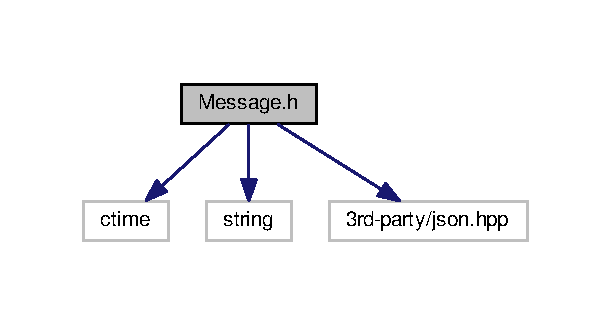
\includegraphics[width=293pt]{Message_8h__incl}
\end{center}
\end{figure}
This graph shows which files directly or indirectly include this file\+:
\nopagebreak
\begin{figure}[H]
\begin{center}
\leavevmode
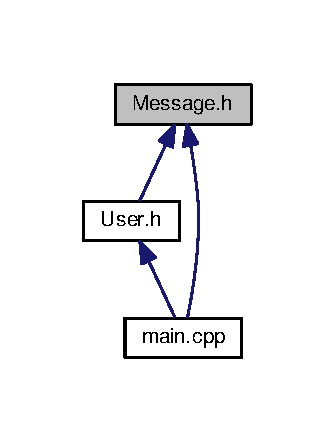
\includegraphics[width=161pt]{Message_8h__dep__incl}
\end{center}
\end{figure}
\subsection*{Classes}
\begin{DoxyCompactItemize}
\item 
struct \hyperlink{structMessage}{Message}
\end{DoxyCompactItemize}
\subsection*{Typedefs}
\begin{DoxyCompactItemize}
\item 
using \hyperlink{Message_8h_af13a1979f9e8f62c101433fac6511cc6}{Json} = nlohmann\+::json
\end{DoxyCompactItemize}
\subsection*{Functions}
\begin{DoxyCompactItemize}
\item 
void \hyperlink{Message_8h_a6c26c6712dcc44d73a0bd41b502a6f57}{to\+\_\+json} (\hyperlink{main_8cpp_af13a1979f9e8f62c101433fac6511cc6}{Json} \&j, const \hyperlink{structMessage}{Message} \&m)
\begin{DoxyCompactList}\small\item\em Called by J\+S\+ON library. \end{DoxyCompactList}\end{DoxyCompactItemize}


\subsection{Typedef Documentation}
\index{Message.\+h@{Message.\+h}!Json@{Json}}
\index{Json@{Json}!Message.\+h@{Message.\+h}}
\subsubsection[{\texorpdfstring{Json}{Json}}]{\setlength{\rightskip}{0pt plus 5cm}using {\bf Json} =  nlohmann\+::json}\hypertarget{Message_8h_af13a1979f9e8f62c101433fac6511cc6}{}\label{Message_8h_af13a1979f9e8f62c101433fac6511cc6}


\subsection{Function Documentation}
\index{Message.\+h@{Message.\+h}!to\+\_\+json@{to\+\_\+json}}
\index{to\+\_\+json@{to\+\_\+json}!Message.\+h@{Message.\+h}}
\subsubsection[{\texorpdfstring{to\+\_\+json(\+Json \&j, const Message \&m)}{to_json(Json &j, const Message &m)}}]{\setlength{\rightskip}{0pt plus 5cm}void to\+\_\+json (
\begin{DoxyParamCaption}
\item[{{\bf Json} \&}]{j, }
\item[{const {\bf Message} \&}]{m}
\end{DoxyParamCaption}
)}\hypertarget{Message_8h_a6c26c6712dcc44d73a0bd41b502a6f57}{}\label{Message_8h_a6c26c6712dcc44d73a0bd41b502a6f57}


Called by J\+S\+ON library. 


\hypertarget{NetworkError_8h}{}\section{Network\+Error.\+h File Reference}
\label{NetworkError_8h}\index{Network\+Error.\+h@{Network\+Error.\+h}}
{\ttfamily \#include $<$cerrno$>$}\\*
{\ttfamily \#include $<$cstring$>$}\\*
{\ttfamily \#include $<$string$>$}\\*
{\ttfamily \#include $<$stdexcept$>$}\\*
Include dependency graph for Network\+Error.\+h\+:
\nopagebreak
\begin{figure}[H]
\begin{center}
\leavevmode
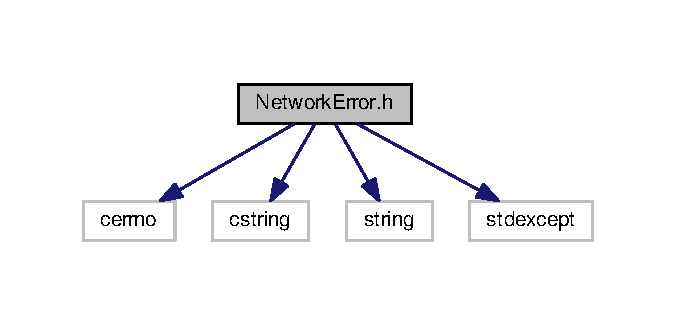
\includegraphics[width=325pt]{NetworkError_8h__incl}
\end{center}
\end{figure}
This graph shows which files directly or indirectly include this file\+:
\nopagebreak
\begin{figure}[H]
\begin{center}
\leavevmode
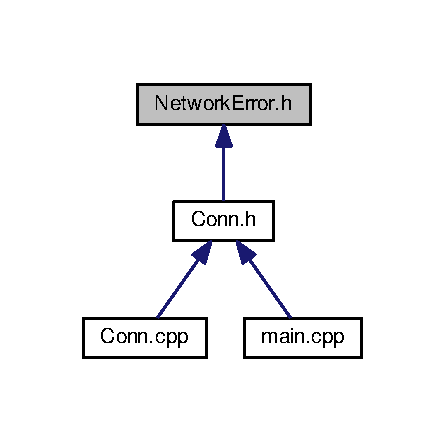
\includegraphics[width=214pt]{NetworkError_8h__dep__incl}
\end{center}
\end{figure}
\subsection*{Classes}
\begin{DoxyCompactItemize}
\item 
class \hyperlink{classNetworkError}{Network\+Error}
\end{DoxyCompactItemize}

\hypertarget{User_8h}{}\section{User.\+h File Reference}
\label{User_8h}\index{User.\+h@{User.\+h}}
{\ttfamily \#include $<$vector$>$}\\*
{\ttfamily \#include $<$string$>$}\\*
{\ttfamily \#include \char`\"{}Message.\+h\char`\"{}}\\*
Include dependency graph for User.\+h\+:
\nopagebreak
\begin{figure}[H]
\begin{center}
\leavevmode
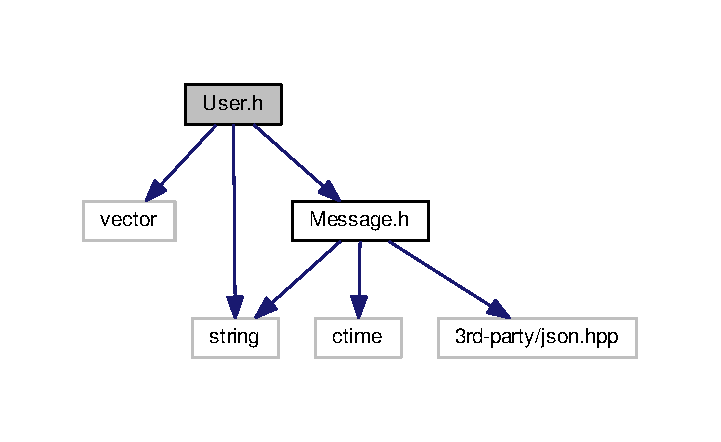
\includegraphics[width=346pt]{User_8h__incl}
\end{center}
\end{figure}
This graph shows which files directly or indirectly include this file\+:
\nopagebreak
\begin{figure}[H]
\begin{center}
\leavevmode
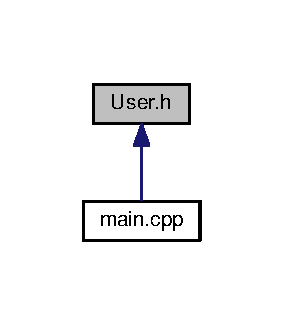
\includegraphics[width=136pt]{User_8h__dep__incl}
\end{center}
\end{figure}
\subsection*{Classes}
\begin{DoxyCompactItemize}
\item 
struct \hyperlink{structUser}{User}
\end{DoxyCompactItemize}

%--- End generated contents ---

% Index
\backmatter
\newpage
\phantomsection
\clearemptydoublepage
\addcontentsline{toc}{chapter}{Index}
\printindex

\end{document}
